\chapter{Simulation environment}
\label{cap:3}In this chapter the endeavor at a more solid validation in terms of the robustness of the simulator will be presented. Firstly, the setup on the simulator will be introduced. Secondly, the necessary setup correlated to the ROS2-BDI framework will be shown. Finally, the overall architecture will be summarized.
\section{Main scenario description}
Three different scenarios were implemented, only the first shall be explained thoroughly as it is the most basic one. The idea is that there is a $7$  by $7$ grid where objects to continue to appear. The robot's goal is to retrieve these objects and to transfer them to a designated place, the bin. Boxes are placed randomly in the arena with the objective to make the robot's life a little harder.
\begin{figure}[H]
\centering
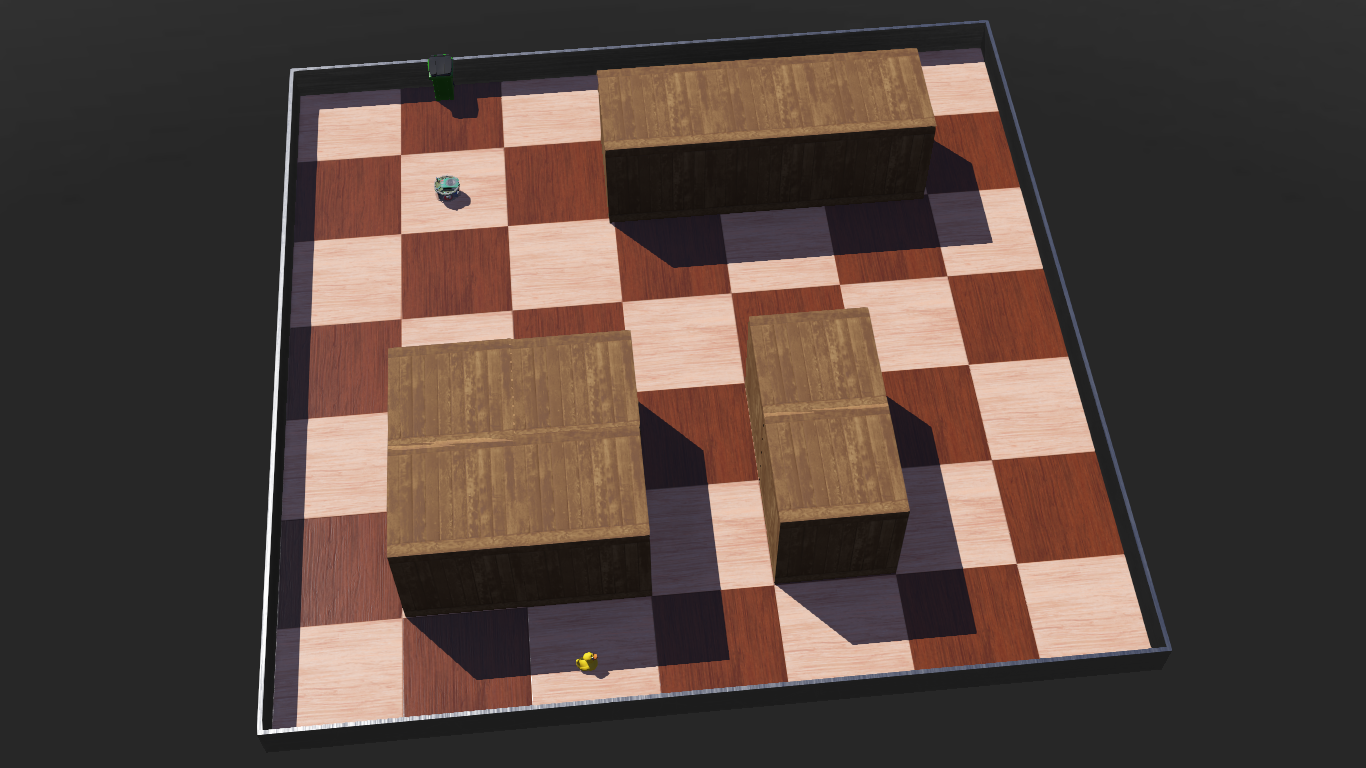
\includegraphics[width=\textwidth]{images/simulation_screen.png}
\caption{Webots simulation in the initial state}
\end{figure}
\section{Webots setup} Let us now look at the necessary steps to take in order to connect the Webots simulator to ROS2, hence enabling it to work with ROS2-BDI.
\par
To begin with, we create a ROS2 package defaulting the node's language to \texttt{Python3} and adding the \texttt{rclpy} library dependency. The original idea was to use \texttt{C++} in order to make the project as consistent as possible with the rest of the implementation, however, the author is not aware of a method which employs the \texttt{C++} language as the official documentation only presents how to use \texttt{Python3}.
\par
A \texttt{setup.py} file needs to be created where all the different resources are declared. These are the world itself, the different robots and the launcher.
\par
Under the \texttt{worlds} directory we need to put the \texttt{.wbt} file which describes what the Webots world looks like.
\par
Inside the \texttt{resources} directory the robot controllers and the supervisor declaration needs to be specified. Here's what the declaration of the main robot looks like: 
\begin{lstlisting}[language=XML, caption=XML file linking robot controller to Webots]
<?xml version="1.0" ?>
<robot name="e_puck">
    <webots>
        <plugin type="spawn_spazza.e_puck_controller.MyRobotDriver" 
        webots_robot_name="e_puck"/>
    </webots>
</robot>
\end{lstlisting}
In line four and five we are specifying the current package \texttt{spawn\_spazza}, the name of the \texttt{Python3} file containing the controller of the robot (\texttt{e\_puck\_controller}) and the name of the class which extends the package needed to create a ROS2 node and which defines the behavior of the robot \texttt{MyRobotDriver}. \texttt{webots\_robot\_name} is used to indicate which robot we are talking about in the simulation.
\par
Now the last step is writing the launcher which is just a file booting up multiple ROS2 nodes. What it does is it enumerates each node to execute, alongside their optional parameters. For example here's what the code launching the robot look like
\begin{lstlisting}[language=Python, caption=launch description for a Webots robot]
        robot_description = pathlib.Path(os.path.join(package_dir, 'resource', 'e_puck.urdf')).read_text()

        my_robot_driver = Node(
        package='webots_ros2_driver',
        executable='driver',
        output='screen',
        additional_env={'WEBOTS_CONTROLLER_URL': controller_url_prefix() + 'e_puck'},
        parameters=[
            {'robot_description': robot_description},
        ],  

        arguments=[
            '--webots-robot-name', 'e_puck',
            '--webots-node-name', 'e_puck'
        ]
    )
\end{lstlisting}
The only thing that is happening here is that we are launching a node whose code is specified inside the \texttt{e\_puck.urdf} file as show above in listing 3.1.
\par
That is all there is to it in the Webots side. Next the implementation of the robot's controller and the supervisor will be discussed.
\section{Robot controller}
\subsection{e\_puck}
The chosen robot was the e\_puck as it is uncomplicated to use and the provided API's are reliable, well documented and work across different languages. 
\par
The e\_puck is a circular robot with seven sensors surrounding it and two wheels on opposite sides controlled by two different motors which can either go forwards or backwards. In order to move forwards it is sufficient to set the speed of both motors to the same positive value. To move backwards the value would need to be negative. Rotating the robot is quite simple as well, we just need to set the speed of the right motor to a positive real value $s$ and $-s$ to the left if we want to rotate anticlockwise. $-s$ and $s$ to rotate clockwise.
\subsection{e\_puck movement mechanisms} Let us now analyze how the movement of the robot works. The e\_puck is placed inside a 3D world with a coordinate system and initially occupies the $(0.0,0.0,0.0)$ position. At some point in the simulation it will receive the order to move to a certain position $(x,y,z)$. The basic idea is to rotate the robot until it faces the target position. Then, move it forwards until it reaches the objective. Here is the pseudocode that shows exactly how this works.
\begin{lstlisting}[language=Python, caption=e\_puck robot movement algorithm]
LEFT = 1, RIGHT = -1
FORWARDS = 1, BACKWARDS = -1
ERROR = 0.01 #error that one is willing to tolerate

def move_robot (robot, pos):
    target_theta = target_theta(robot, pos)
    direction = direction(robot, pos)

    while (abs(robot.theta - target_theta) > ERROR):
        rotate_robot(direction)
    
    while (dist(robot, pos) > ERROR):
        move_robot(FORWARDS)
\end{lstlisting}
\texttt{LEFT}, \texttt{RIGHT}, \texttt{FORWARDS} and \texttt{BACKWARDS} are all constants defined in order to make the code cleaner. While \texttt{ERROR} serves as a way of allowing a small degree of imperfection. 
\par
The implementation of the \texttt{target\_theta} and \texttt{direction} functions are just as fascinating. Let us go over their logic. Before that though we must go through the convention adopted by Webots for the orientation. In the first and second quadrants the angle is defined the same way as it is in mathematics: it starts from $0$ radians and increments all the way to $\pi$ at the end of the second quadrant. The moment it crosses the second quadrant and goes into the third the angle goes from $+\pi$ to $-\pi$, after that it decreases all the way to $0$. Here is a picture to better explain the convention.
\begin{figure}[H]
\centering
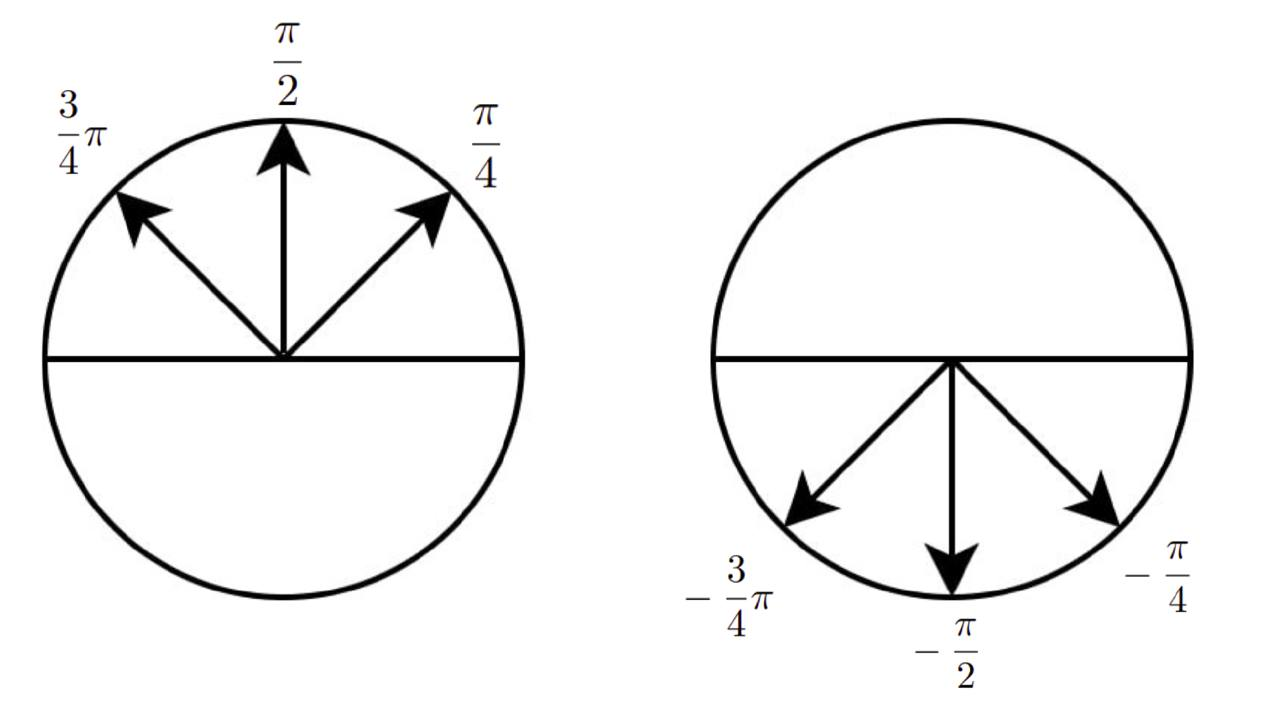
\includegraphics[scale=0.2]{images/webots_angles.jpg}
\caption{Webots orientation convention}
\end{figure}
To rotate the robot towards the objective we start by calculating $\Delta y$ and $\Delta x$ which are respectively the difference in the $y$ and $x$ coordinates between the target and the robot. Under normal circumstances the angle between the robot and the target is defined as $\arctan (\frac{\Delta y}{\Delta x})$. That is because we know from trigonometry that the tangent of $\theta$ is equal to the ratio between the opposite and adjacent side.
\cite{analisi1}
\par
Depending on the sign of $\Delta x$ and $\Delta y$ we split in to four cases:
\newpage
\textbf{$\Delta y > 0 \quad and \quad \Delta x > 0$}: \\ 
\begin{minipage}{0.4\textwidth}
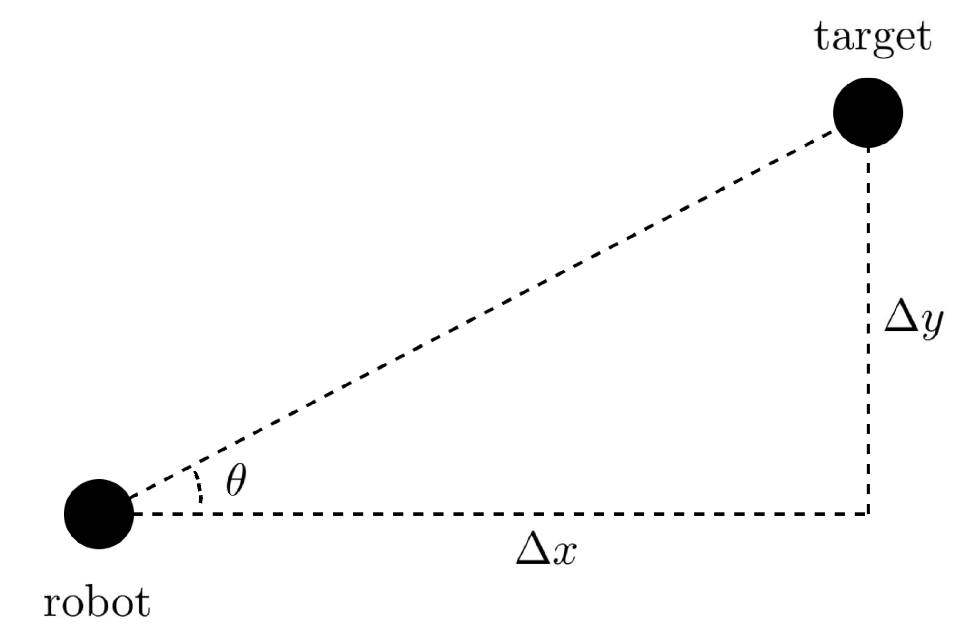
\includegraphics[width=\linewidth]{images/theta1.jpg}
\end{minipage}
\begin{minipage}{0.5\textwidth}\raggedleft
$$\quad \quad \quad \quad \theta = \arctan\left(\frac{\Delta y}{\Delta x}\right)$$ \\
\end{minipage}
\noindent
\\
In this case we simply take the angle between the robot and the target.
\\
\\
\textbf{$\Delta y > 0 \quad and \quad \Delta x < 0$}: \\ \\
\begin{minipage}{0.4\textwidth}
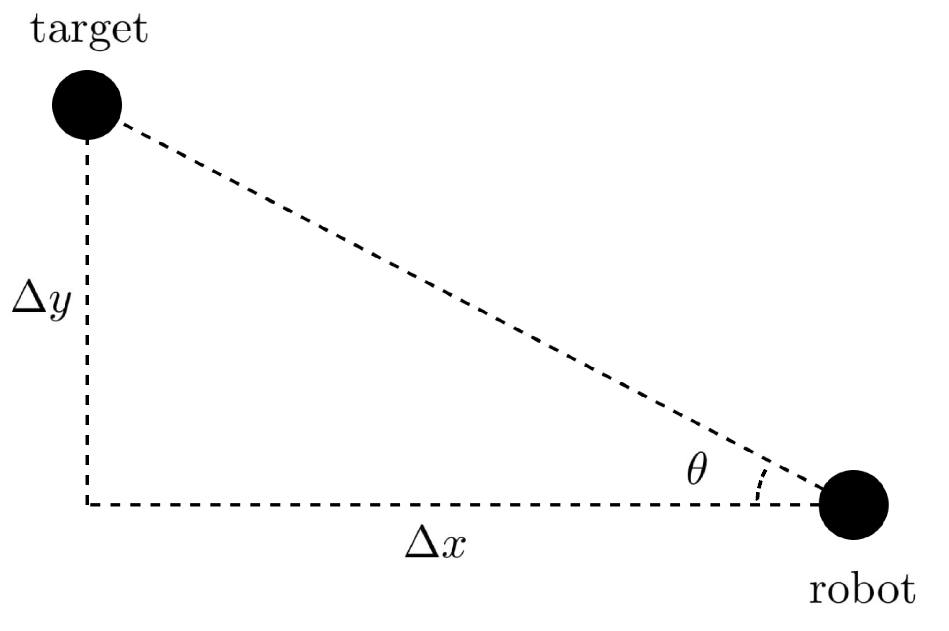
\includegraphics[width=\linewidth]{images/theta2.jpg}
\end{minipage}
\begin{minipage}{0.5\textwidth}\raggedleft
$$\quad \quad \quad \quad \theta = \pi - \left| \arctan\left(\frac{\Delta y}{\Delta x}\right) \right|$$ \\
\end{minipage}
\noindent
\\
The formula here takes $\pi$ and subtracts to it the angle between the robot and target because we want to take the full $180$ degrees minus the quantity show in the picture, which is $\theta$.
\\
\\
\textbf{$\Delta y < 0 \quad and \quad \Delta x < 0$}: \\ \\
\begin{minipage}{0.4\textwidth}
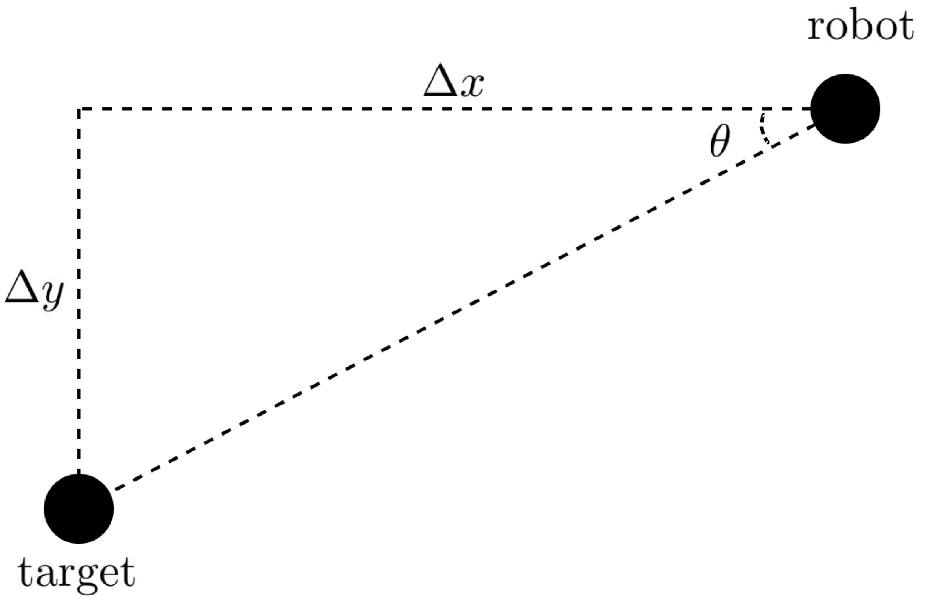
\includegraphics[width=\linewidth]{images/theta3.jpg}
\end{minipage}
\begin{minipage}{0.5\textwidth}\raggedleft
$$\quad \quad \quad \quad \theta = \frac{\pi}{2} -  \left| \arctan\left(\frac{\Delta x}{\Delta y}\right) \right|$$ \\
\end{minipage}
\noindent
\\
$\Delta x$ and $\Delta y$ get swapped because when moving upside down so do the opposite and adjacent sides.
\\
\\
\textbf{$\Delta y < 0 \quad and \quad \Delta x > 0$}: \\ \\
\begin{minipage}{0.4\textwidth}
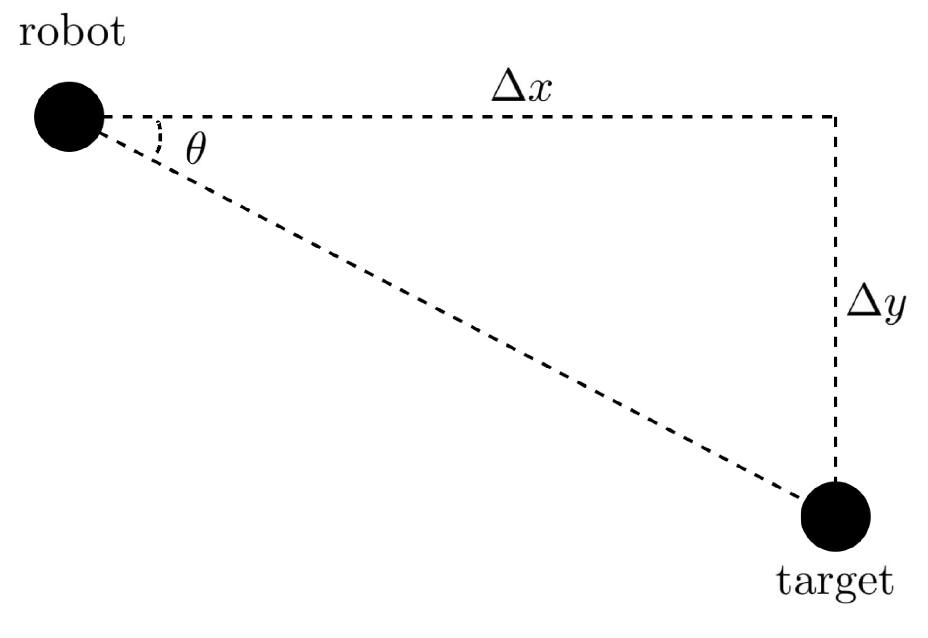
\includegraphics[width=\linewidth]{images/theta4.jpg}
\end{minipage}
\begin{minipage}{0.5\textwidth}\raggedleft
$$\quad \quad \quad \quad \theta = \frac{\pi}{2} + \left| \arctan\left(\frac{\Delta x}{\Delta y}\right) \right|$$ \\
\end{minipage}
\noindent
\\
The idea behind that $- \frac{\pi}{2}$ is that we want to take $90$ degrees plus the angle between the robot and the target. One quick look at the diagram will convince us of that. 
\par 
Now let us briefly explore the idea behind the \texttt{direction} function. The objective of this function is to decide whether to turn the robot left or right. As a reminder, by robot's orientation we mean the direction the robot is facing, while the target's angle is the angle which the robot should be orientated to in order to be headed towards the target. In a similar fashion to the \texttt{target\_theta} function, we split into four cases:
\begin{enumerate}
    \item Both the robot and \texttt{target\_theta} have a positive orientation. In this case we turn left if the robot's angle is smaller, right otherwise.
    \item Both are negative. Coincidentally the behavior in this case is the same as before.
    \item The robot's orientation is positive and the target's angle is negative. What we do here is calculate by how much we would have to move if we were to go both left and right. Right: we sum the angle of the robot and we subtract to it the angle of the target. Left: We take $\pi$ and remove the angle of the robot, then we add $\pi$ again and add the angle of the target. Only checking which one of this two quantities is bigger is left in order to decide where to go. The idea behind this case will be clearer when looking at the code.
    \item The robot's orientation is negative and the target's positive. We apply the same trick but we invert the decision we take. In other words if the first quantity is bigger than the second we turn left, right otherwise.
\end{enumerate}
As promised, here is the the algorithm which will hopefully clear things up.
\begin{lstlisting}[language=Python, caption=algorithm which decides whether to rotate RIGHT or LEFT]
def direction(robot, target): 
    #first and second case
    if robot.theta >= 0 and target.theta >= 0 or robot.theta <= 0 and target.theta <= 0:
        return LEFT if robot.theta < target.theta else RIGHT 
    
    #third case
    if robot.theta >= 0 and target.theta <= 0:
        right = robot.theta - target.theta
        left = 2 * math.pi - robot.theta + target.theta
        return RIGHT if right < left else LEFT

    #fourth case
    right = robot.theta - target.theta
    left = 2 * math.pi - robot.theta + target.theta
    return LEFT if right < left else RIGHT
\end{lstlisting}
\subsection{ROS2 communications}
The e\_puck robot is associated to the following ROS2 topics:
\begin{itemize}
    \item \textbf{\texttt{e\_puck/move}}: (subscriber). The message is an integer. It indicates the tile the robot should move to (to every tile a unique integer is assigned). It is the ROS2-BDI framework who publishes to this topic of course.
    \item \textbf{\texttt{e\_puck/position}}: (subscriber).The message contains four floats: the $x$, $y$, $z$ coordinates and the orientation $theta$. The supervisor publishes to this topic
    \item \textbf{\texttt{e\_puck/move\_completed}}: (publisher). The message is of empty type. It serves the purpose to indicate that the requested move was completed. Note that a service could have been used instead in this case.
\end{itemize}

\section{Supervisor} 
The supervisor is, at its core, a normal Webots robot. What makes it special is the ability to create and destroy new objects, access the parameters of other robots and objects (such as translation, orientation, scale, color, ecc...) and automatically subscribe to the simulation ROS2 topic \texttt{/clock}, which gives a very accurate estimation of how much time has elapsed since the beginning of the simulation.
\subsection{Purpose}
The purpose of the supervisor in this simulation is to:
\begin{itemize}
    \item Spawn new ducks every $n$ seconds and to remove the ducks whose internal clock has timed out. 
    \item Publish to the \texttt{e\_puck/position} topic the current position and orientation of the robot. Note that the e\_puck itself does not have access to its position, for this reason going through the supervisor to get this information is the only way to go. An alternative solution could have been to attach a GPS device to the robot, but to the author's mind it would have been a bit too convoluted of a solution. Besides, this would have implied not having access to the orientation, for the GPS does not provide that kind of information. 
    \item Publish to the \texttt{e\_puck/add\_belief} and \texttt{e\_puck/del\_belief} topics which indicate to the ROS2-BDI instance that a belief has to be added or deleted. This is necessary because ROS2-BDI needs to know where new ducks are spawned and if they get deleted.
\end{itemize}
\section{ROS2-BDI}
Let us walk through the general setup which would allow us to connect the Webots simulation to the ROS2-BDI instance correctly. Here is what needs to be done specifically: 
\begin{itemize}
    \item Setup the \textbf{initial beliefs}.
    \item Optionally, define an initial \textbf{desire set}.
    \item Optionally, designate the \textbf{reactive rules}.
    \item Create a \textbf{PDDL 2.1 domain}.
    \item Create the node definition for the \textbf{actions} specified in the domain definition.
    \item Optionally, describe the \textbf{sensors}, if any.
    \item Generate a \textbf{launcher} which will instantiate ROS2-BDI and the action/sensor nodes. 
\end{itemize}
What is going on, fundamentally, is that the framework will look at the domain and come up with a plan to satisfy the desires accordingly. The plan will be then executed thanks to the definitions of the actions. Furthermore the reactive rules, if defined, will be followed whenever necessary.
\subsection{PDDL domain}
Before all else we need to define the objects our world contains. These are the robot, the garbage, the box, the tile and the bin. Note that the tile represents a square in which objects can be positioned in the simulation. We can do exactly that by typing:  
\begin{lstlisting}[caption=PDDL 2.1 domain]
~;; Types ;;;;;;;;;;;;;;;;;;;;;;;;;;;;;;~
    (:@types@
        robot garbage box tile bin
    )~;; end Types ;;;;;;;;;;;;;;;;;;;;;;;;;~
\end{lstlisting}
Now the predicates (i.e. the statements about the world which can either be true or false):
\begin{lstlisting}[caption=Predicates definition]
(:@predicates@
    (at_rob ?r - robot ?t - tile)
    (at_gar ?g - garbage ?t - tile)
    (at_box ?b - box ?t - tile)
    (at_bin ?b - bin ?t - tile)
    (free ?r - robot)
    (adjacent ?t1 - tile ?t2 - tile)
    (walkable ?t - tile)
    (holding ?r - robot ?g - garbage)
    (deleted ?g - garbage)
    (to_recycle ?g - garbage)
)
\end{lstlisting}
Here is an explanation of the predicates:
\begin{itemize}
    \item \texttt{at\_x} indicates that the object of type \texttt{x} is located at tile $t$.
    \item \texttt{free} to say the robot is free and not holding anything.
    \item \texttt{adjacent} specifies that \texttt{t1} and \texttt{t2} are close to each other. This was done to lighten the work on the simulation side and let the ROS2-BDI program do the work. In fact if this condition was not there the move function would be orders of magnitude more complicated.
    \item \texttt{walkable} is used to mark tiles as either walkable or unwalkable. A tile cannot be crossed if an object or a box is on top of it.
    \item \texttt{holding} designates that the robot \texttt{r} is holding the piece of garbage \texttt{g}.
    \item When the supervisor deletes an object because it timed out the \texttt{deleted} predicate is set to true for that specific object.
    \item When an object has just been spawned, the \texttt{to\_recycle} predicate is initialized to true, which indicates that \texttt{g} needs to be collected and brought to the bin.
\end{itemize}
Only three actions are necessary to describe the simulation. These are \texttt{move}, \texttt{pickup} and \texttt{putdown}.
\begin{lstlisting}[caption=move action definition]
(:@durative-action@ move
    :@parameters@ (?r - robot ?from ?to - tile)
    :@duration@ (= ?duration 3)
    :@condition@ (and 
        (at start (at_rob ?r ?from))
        (over all (adjacent ?from ?to))
        (over all (walkable ?to))
    )
    :@effect@ (and
        (at start (not(at_rob ?r ?from)))
        (at end (at_rob ?r ?to))
    )
)
\end{lstlisting}
This action moves the robot from one tile to another. The preconditions require the robot to be at the starting tile in the beginning. What's more it is paramount the the destination tile is walkable and adjacent to the source tile. The effect is quite trivial: at the beginning the robot is not located at the source tile anymore and at the end it is situated at the destination one.
\begin{lstlisting}[caption=pickup action definiton]
(:@durative-action@ pickup
    :@parameters@ (?r - robot ?t - tile ?g - garbage)
    :@duration@ (= ?duration 1)
    :@condition@ (and
        (at start(free ?r))
        (at start (at_gar ?g ?t))
        (at start (at_rob ?r ?t))
    )
    :@effect@ (and
        (at end (not(free ?r)))
        (at end (not(at_gar ?g ?t)))
        (at end (holding ?r ?g))
    )
)
\end{lstlisting}
This action represent the moment where the robot picks up an object. For it to happen it is necessary that the robot and the object share the same position and for the robot to be free (i.e. not holding other objects). The effect is also self explanatory: the robot is not free anymore and is holding the object. The garbage is no longer positioned at its initial position.
\begin{lstlisting}[caption=Putdown action definition]
(:@durative-action@ putdown
    :@parameters@ (?r - robot ?t - tile ?b - bin ?g - garbage)
    :@duration@ (= ?duration 1)
    :@condition@ (and
        (over all (at_bin ?b ?t))
        (over all (at_rob ?r ?t))
        (at start (holding ?r ?g))
    )
    :@effect@ (and
        (at end(free ?r))
        (at end(at_gar ?g ?t))
        (at end (not(holding ?r ?g)))
    )
)
\end{lstlisting}
This action describes the act of the robot putting down an object. As a precondition it is obligatory that the robot holds the object and that the bin and the robot are located at the same tile. The effect is that the robot is now free and no longer holding on to anything. Furthermore the object is now at its destination.
\subsection{Belief set initialization}
To make sure that the ROS2-BDI instance behaves faithfully to the PDDL domain it is critical to initialize the set of predicates believed to be true at the beginning of the simulation. Additionally all the objects (robot, tile, box....) need to defined. All these beliefs need to be inserted into a \texttt{.yaml} file, respecting the syntax that will be shown.
\par
First things first, let us go over all the objects that need to be defined. 
\begin{itemize}
    \item The e\_puck robot.
    \item The bin
    \item All the boxes.
    \item All the $49$ tiles, named from \texttt{t0} to \texttt{t48}.
\end{itemize}
It is quite straightforward to write this kind of declaration inside the \texttt{.yaml} file. For example if we wanted to declare the e\_puck robot we would write:
\begin{lstlisting}
- @name@: "e_puck"
  @pddl_type@: 1
  @type@: "robot"
\end{lstlisting}
A \texttt{pddl\_type = 1} indicates that we are discussing an object declaration, while a \texttt{pddl\_type = 2} means we are working with a predicate.
\par
Now, onto the predicates initialization:
\begin{itemize}
    \item The position of the robot, the bin and the boxes.
    \item The robot must be initialized as free by setting the \texttt{free} predicate to \texttt{true}.
    \item Each tile which does not contain a box or any other object needs to be declared as \texttt{walkable}.
    \item For each tile all of its adjacencies ought to be itemized. For simplicity's sake only the up, down, right and left directions were considered, while the diagonals were not taken notice of. This can be done by making use of the \texttt{adjacent} predicate.
\end{itemize}
Once again, the syntax for this kind of statement is trivial. Say we wanted to show that the tile \texttt{t1} and \texttt{t3} are adjacent. To do that the following piece of code would be sufficient.
\begin{lstlisting}
- @name@: "adjacent"
  @pddl_type@: 2
  @params@: 
    - "t1"
    - "t3"
- @name@: "adjacent"
  @pddl_type@: 2
  @params@: 
    - "t3"
    - "t1"
\end{lstlisting}
It is needed to declare both \texttt{t1} adjacent to \texttt{t3} and vice versa because the planner may be checking the predicate from either side.
\subsection{Reactive rules}
Reactive rules allow us to dynamically modify the belief and desire sets via some predefined rules. They are optional but a very nice to have feature and essential for some scenarios. The first scenario does not actually need reactive rules, however, the second scenario, in which ducks appear as well as disappear, finds them vital. Consequently let us go through them. We only need two of them: One that pushes the desire to retrieve objects whenever they appear and one to delete the desire to retrieve the objects that have timed out. Like belief and desire set initialization, they are defined inside a \texttt{.yaml} file.
\begin{lstlisting}[caption=Reactive rule that pushes the desire to retrieve an object as soon as it spawns]
- @condition@:
    @clauses@:
    - @literals@:
        - @check@: "EX"
            @condition_to_check@:
            @name@: "{x}"
            @pddl_type@: 1
            @type@: "garbage"
      
        - @check@: "T"
            @condition_to_check@:
            @name@: "to_recycle"
            @pddl_type@: 2
            @params@:
                - "{x}"
      
        - @check@: "F"
            @condition_to_check@:
            @name@: "deleted"
            @pddl_type@: 2
            @params@:
                - "{x}"

@reactive_rules@: 
    - @set@: desire
    @operation@: ADD
    @value@:
        @name@: "recycle_{x}"
        @priority@: 0.6
        @deadline@: 1000
        @value@:
        - @name@: "at_gar"
          @pddl_type@: 2
          @params@:
            - "{x}"
            - "t1"
\end{lstlisting}
Basically if the first three checks are verified at any point in time the reactive rule condition is set off. The first condition checks whether an object of type garbage exists; the second whether it needs to be recycled or not and the third makes sure it has not been deleted already. If all three conditions are satisfied the desire to retrieve the object and put it next to the bin is pushed. Now, Let us look at the second reactive rule.
\begin{lstlisting}[caption=Reactive rule that deletes the desire to retrieve an object if it no longer exists]
- @condition@:  
    @clauses@:
      - @literals@:
        - @check@: "T"
          @condition_to_check@:
            @name@: "deleted"
            @pddl_type@: 2
            @params@:
              - "{x}"

  @reactive_rules@:
    - @set@: desire
      @operation@: DEL
      @value@:
        @name@: "recycle_{x}" 
        @priority@: 0.6
        @deadline@: 1000
        @value@:
          - @name@: "at_gar"
            @pddl_type@: 2
            @params@:
              - "{x}"
              - "t1"    
\end{lstlisting}
If the \texttt{deleted} predicate is true for the object \texttt{\{x\}} then the reactive rule's execution is triggered. As a result of that the desire to recycle that object is removed from the \texttt{belief\_set}.
\subsection{Actions}
One action is defined for each durative action inside the PDDL domain, that means move, pickup and put down. The definition is embedded inside a ROS2 node, which is especially convenient as it allows the use of ROS2 functionalities inside of it. Basically the idea is to use ROS2 communication tools to contact the simulation and tell it what to do. The advantageous thing of this is that everything will take care of itself automatically as the action execution is triggered autonomously by the ROS2-BDI instance. In other words if the planner believes that the best course of action in a certain time step of the simulation is to perform a move action, ROS2 topics and services will be called from inside the action node definition and will tell the robot to move to the designated tile.
\par
Let us look at the definition of one of these actions, the move action.
\begin{lstlisting} [language=c++, caption=Move action node]
class Move : public BDIActionExecutor {
public:
    Move() : BDIActionExecutor("move", 1) {
        publisher_ = this->create_publisher<std_msgs::msg::Int16>("move", 10);

        subscriber_ = this->create_subscription<std_msgs::msg::Empty>(
            "move_completed", 4,
            std::bind(&Move::move_completed_callback, this, _1));

        publisher_->on_activate(); // activate publisher on node creation
    }

    float advanceWork() {
        publisher_->publish(create_msg());

        if (move_completed) {
            move_completed = false;
            return 1.0f;
        }

        return 0.025f;
    }

    void move_completed_callback(const std_msgs::msg::Empty::SharedPtr msg) {
        move_completed = true;
    }

    std_msgs::msg::Int16 create_msg() {
        std::vector<std::string> arguments = this->getArguments();

        auto msg = std_msgs::msg::Int16();
        msg.data = arguments[2][1] - '0'; // -'0' trick to convert char to int
        if (arguments[2][2] >= '0' && arguments[2][2] <= '9')
            msg.data = (arguments[2][1] - '0') * 10 + (arguments[2][2] - '0');
        
        return msg;
    }
};
\end{lstlisting}
In the constructor the node is instantiating the publisher for the \texttt{/move} topic. This node will be told from ROS2-BDI when to activate and when it happens it will publish to the \texttt{/move} topic. It also subscribes to the \texttt{/move\_completed} topic in case the e\_puck terminates its movement earlier than anticipated. 
\par
The constructor's parameter \texttt{"move"} is used this node to the right action. The parameter \texttt{1} is used to decide how many times a second the method \texttt{advanceWork()} is called.
\par
The method \texttt{advanceWork()}, which in this case is called $1$ time per second, is used as the feedback of the action by returning a float. The action will be considered uncompleted until the cumulative return values of the \texttt{advanceWork()} will be less than $1$. The function is defined in a similar fashion to a state machine: it keeps returning \texttt{0.025f}, but if the flag \texttt{completed} is true (which happens if a message arrives from the \texttt{move\_completed} topic) it returns \texttt{1.0f}. The value \texttt{0.25f} was set because the move action is believed to last at most $40$ seconds, therefore either the action concludes naturally at the end of this time period or it interrupts earlier due to the flag being set to \texttt{true}.
\par
The method \texttt{advanceWork()} main job is to publish to the topic \texttt{e\_puck/move}, which it does at the line number $14$. The message could be sent up to $40$ times but it will not be an issue since the extra messages will by no means impede the e\_puck's calculations. The message contains the tile towards which the robot should move. It is calculated thanks to the API call \texttt{getArguments()} which contains the name of the action and its parameters.
\subsection{Launcher} In the ROS2-BDI architecture the launcher's main job is to instantiate the core node's and make the necessary connections to the actions automatically. In addition to that it allows the user to define some key parameters such as the planning configuration (online or offline), the reschedule policy, the beliefs \texttt{.yaml} file, the reactive rules \texttt{.yaml} file and other less interesting parameters for this particular simulation. The aforementioned parameters were the main ones played with across each different scenario. 
\subsection{Overall architecture} 
As promised at the beginning of this chapter, here is the overall architecture for this simulation:
\begin{figure}[H]
\centering
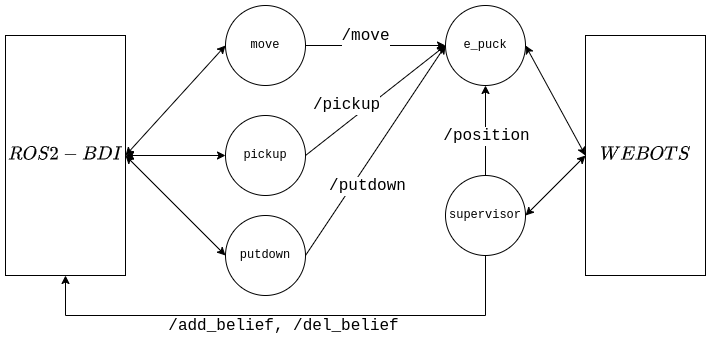
\includegraphics[width=\textwidth]{images/simulation_architecture.png}
\caption{The simulation's architecture}
\end{figure}
The two big rectangles are the representation of the ROS2-BDI instance and the Webots instance. The circles are ROS2 nodes and they communicate with each other using ROS2 communications. Unidirectional arrows represent ROS2 topics, while bidirectional arrows are either ROS2 services or actions. 
\par
The three nodes \texttt{move}, \texttt{pickup} and \texttt{putdown} are automatically generated by ROS2-BDI when launching and exchanged messages are handled autonomously by the ROS2-BDI architecture. They instruct the robot e\_puck robot when to perform those actions with the depicted topics.
\par 
The e\_puck node reads the messages from the action topics and leverages the Webots API which are implemented upon ROS2 to tell the graphical simulation to perform the requested action. The name of these ROS2 communications are omitted, for they are hidden to the programmer since Webots API's handle everything on the background. They are however indicated in the diagram unnamed. A clarification is needed here, the messages are used just to turn instruct the graphical interface to turn the motors, not to indicate an abstract action such as \texttt{move t2}.
\par
The supervisor gets the information about the world from the Webots instance thank to the provided API's implemented on top of ROS2. It publishes to the topic \texttt{/position} which indicates the position of the robot. Furthermore it publishes to the topics \texttt{add\_belief} and \texttt{del\_belief} whenever a new objects appears and disappears. It is the supervisor's job to handle the belief set for this kind of action because it is also responsible of spawning and deleting new objects.
\newpage
